% Converted from MITS_26MPE05015_IEEE_Manuscript.docx.
% Uses the JPP LaTeX structure supplied by the user; requires jpp.cls.
% The logo is cropped from the university image supplied by the user.
\documentclass{jpp}
\usepackage[utf8]{inputenc}
\usepackage[T1]{fontenc}
\usepackage{graphicx}
\usepackage{amsmath}
\shorttitle{Adversarial ECG camouflage and recovery}
\shortauthor{M. S. varma and S. dash}
\title{
\includegraphics[height=1.45cm]{figures/mits_logo.png}\\[0.8ex]
Adversarial ECG Camouflage with Authenticated Recovery and Residual Attention Classification}
\author{Muddisetty Sreekar varma\aff{1} \and Sachikanta dash\aff{1}}
\affiliation{\aff{1}MITS -- Deemed to be University \\
(Madanapalle Institute of Technology \& Science), Madanapalle, Andhra Pradesh, India}
\begin{document}
\maketitle
\begin{abstract}


We present a local research workbench that combines electrocardiogram rhythm classification, adversarial signal camouflage, and authenticated recovery of original MATLAB recordings. A compact one-dimensional residual-attention network processes 1,000 ten-second MLII fragments from a public 17-class dataset. The reconstructed 800/200 fragment split gives 87.00\% accuracy and 86.22\% weighted F1; all validation recording identifiers overlap training and three validation waveforms are exact training duplicates. These figures therefore describe leakage-affected internal validation, not unseen-patient performance. A gradient-guided routine changes a publicly readable waveform while an AES-256-GCM payload retains the complete original file. Authenticated creation-time reports show changed predictions for all 1,000 fragments under one known checkpoint, and a separate cryptographic recheck confirms exact MAT recovery for every fragment. An independent normalized-input FGSM experiment reduces validation accuracy to 59.50\% at epsilon 0.05. The study separates classifier sensitivity from cryptographic confidentiality: decoy misclassification is neither attack prevention nor anonymization. The implementation provides a reproducible demonstration of altered-signal prediction and lossless original recovery, without claiming the PPO-based defenses of the RNAF reference framework.

\end{abstract}
\noindent\textbf{Keywords:} Electrocardiography, adversarial examples, authenticated encryption, residual attention, signal classification, reproducibility.


\section{Introduction}

ECG research applications often display a waveform, a predicted rhythm, and a model score on the same screen. When adversarial modification and encryption are added, these representations can be confused. A waveform that receives a different label is still numerical signal data; an encrypted file is a byte sequence that should be authenticated and decrypted before ordinary inference. This distinction is central to the present workbench.

We investigate this distinction using the public ECG signals dataset of Plawiak \cite{plawiak2017}, derived from the MIT-BIH Arrhythmia Database \cite{moody2001}. The application reads MATLAB files directly, predicts one of 17 dataset labels, and visualizes the original, public camouflaged, and restored signals. The source files remain unchanged. A password unlocks the protected original rather than attempting to reverse the adversarial perturbation.

The motivation comes from RNAF, which combines image-based adversarial analysis with reinforcement-learning defenses \cite{rizwan2025}. Its fish-to-dog illustration demonstrates changed model behavior under input manipulation. Our implementation adapts that experimental idea to one-dimensional ECG signals, but does not implement RNAF's PPO policy, adaptive steganalysis, or CIFAR-10 image pipeline. We use the reference to motivate a clearly scoped experiment, not to claim equivalent architecture or results.

The contributions are an integrated three-stage ECG comparison, a raw-waveform camouflage heuristic evaluated through the actual preprocessing chain, and an authenticated container that restores exact original MAT bytes. We also report a dataset-leakage audit and distinguish whole-dataset camouflage outcomes from the baseline validation experiment. The objective is a transparent research prototype, not a deployable clinical diagnosis or privacy system.

\section{Related Work}

Goodfellow et al. introduced the fast gradient sign method (FGSM), which uses an input-loss gradient to construct adversarial examples \cite{goodfellow2015}. Madry et al. developed a robust-optimization perspective and stronger iterative attacks \cite{madry2018}. These works motivate sensitivity testing, but changing a classifier output is not the same operation as encrypting a recording. A readable perturbed waveform does not acquire a confidentiality guarantee merely because its predicted class changes.

RNAF studies digital images using a combination of adversarial training, PPO-based adaptive defense, and steganalysis \cite{rizwan2025}. Its task, data, and threat model differ from our ECG demonstration. We do not directly compare their reported accuracy with our 17-class results, because such a comparison would mix datasets, splits, models, and attacks. The present camouflage update is also not exact projected gradient descent through the raw preprocessing chain.

\begin{table}
\centering
\caption{Distinct roles of the implemented components}\label{tab:roles}
\small
\begin{tabular}{p{0.22\linewidth}p{0.30\linewidth}p{0.30\linewidth}}
\hline
Component & Role & Does not establish \\
\hline
Residual-attention CNN & 17-class prediction & Clinical diagnosis \\
Raw camouflage & Public label-change experiment & Confidentiality \\
FGSM test & Input sensitivity measurement & Universal robustness \\
AES-GCM recovery & Protected exact-original storage & Safety of public decoy \\
RNAF reference \cite{rizwan2025} & Image-defense motivation & Implemented PPO defense \\
\hline
\end{tabular}
\end{table}

For file protection, we use AES-GCM, an authenticated-encryption mode specified by NIST \cite{dworkin2007}. For model visualization, the workbench can generate one-dimensional Grad-CAM relevance maps based on gradients and feature activations \cite{selvaraju2019}. Those maps indicate model-dependent relevance, not validated clinical landmarks. Table~\ref{tab:roles} summarizes the roles of these components without implying that they provide interchangeable security properties.

\section{Dataset and Classification Baseline}

\subsection{Data representation and class support}

The Mendeley Data version 3 release contains 1,000 ten-second MLII fragments sampled at 360 Hz, with 3,600 samples per file and 17 rhythm or pattern categories \cite{plawiak2017}. The release describes recordings from 45 patients and is distributed under CC BY 4.0. Our local loader reads the numeric val array and derives the reference class from its parent folder. These labels are not 17 independent cardiovascular disease diagnoses. Table~\ref{tab:support} reports the actual local class counts and reconstructed validation support.

\begin{table}
\centering
\caption{Local dataset support and validation recall}\label{tab:support}
\small
\begin{tabular}{lccc}
\hline
ID and label & All & Val. & Recall \% \\
\hline
1 NSR & 283 & 57 & 89.5 \\
2 APB & 66 & 13 & 76.9 \\
3 AFL & 20 & 4 & 100.0 \\
4 AFIB & 135 & 27 & 100.0 \\
5 SVTA & 13 & 3 & 0.0 \\
6 WPW & 21 & 4 & 100.0 \\
7 PVC & 133 & 26 & 73.1 \\
8 Bigeminy & 55 & 11 & 90.9 \\
9 Trigeminy & 13 & 3 & 33.3 \\
10 VT & 10 & 2 & 100.0 \\
11 IVR & 10 & 2 & 50.0 \\
12 VFL & 10 & 2 & 100.0 \\
13 Fusion & 11 & 2 & 0.0 \\
14 LBBBB & 103 & 21 & 100.0 \\
15 RBBBB & 62 & 12 & 91.7 \\
16 SDHB & 10 & 2 & 100.0 \\
17 PR & 45 & 9 & 100.0 \\
\hline
\end{tabular}
\end{table}

Abbreviations follow the dataset folders: NSR, normal sinus rhythm; APB, atrial premature beat; AFL, atrial flutter; AFIB, atrial fibrillation; SVTA, supraventricular tachyarrhythmia; WPW, Wolff-Parkinson-White pattern; PVC, premature ventricular contraction; VT, ventricular tachycardia; IVR, idioventricular rhythm; VFL, ventricular flutter; LBBBB/RBBBB, left/right bundle branch block beat; SDHB, second-degree heart block; and PR, pacemaker rhythm. Fusion denotes fusion of ventricular and normal beats.

\subsection{Preprocessing and network architecture}

The preprocessing function applies a fourth-order 0.5-45 Hz Butterworth band-pass with forward-backward filtering. Each fragment is centered by its median and scaled by 1.4826 times its median absolute deviation, using a floor of $10^{-6}$. Every fourth sample is retained, producing 900 normalized input values at 90 Hz. The classifier operates on these values, not on the plotted PNG. The cutoff lies at the downsampled Nyquist frequency; the current implementation has no separate resampling filter, which is a limitation for future signal-processing refinement.

The custom RAMNV2 model contains 27,633 trainable parameters. It uses a convolutional stem, depthwise/pointwise residual blocks, channel attention, temporal average pooling, and a 17-output linear layer. It is inspired by efficient mobile-network principles rather than being a standard MobileNetV2 image backbone. Within each residual block, a kernel-five depthwise convolution is followed by normalization and ReLU, a pointwise convolution, normalization, channel weighting, and a residual addition. The attention gate pools across time, reduces channels, applies ReLU, expands channels, and applies a sigmoid.

\begin{table}
\centering
\caption{Classifier stages for one input fragment}\label{tab:stages}
\small
\begin{tabular}{lcc}
\hline
Stage & Channels & Length \\
\hline
Normalized input & 1 & 900 \\
Kernel-7 stem, stride 2 & 32 & 450 \\
Residual blocks, strides 1 and 2 & 32 & 225 \\
Pointwise channel expansion & 64 & 225 \\
Residual blocks, strides 1, 2, 1 & 64 & 113 \\
Temporal average pooling & 64 & 1 \\
Linear logits & 17 & 1 \\
\hline
\end{tabular}
\end{table}

\subsection{Training provenance and split audit}

The recorded training command used 30 epochs and batch size 32. The implementation uses cross-entropy and AdamW with learning rate 0.001 and weight decay 0.0001. The legacy checkpoint stores the state dictionary, class count, and label map, but does not retain its training configuration. Seed 42 and the stratified 80/20 split are reconstructed from the original defaults; they reproduce the saved accuracy and weighted metrics exactly. This provenance distinction prevents later metadata-saving code from being retrospectively attributed to the earlier checkpoint.

The reconstruction yields 800 training and 200 validation fragments. All 44 filename-derived validation recording identifiers also occur in training, and all 200 validation fragments consequently belong to overlapping recordings. Three validation waveforms exactly match training waveforms. Recording identifiers are proxies rather than independently verified patient identities. The reported validation scores therefore cannot estimate generalization to unseen recordings or patients.

\section{Camouflage and Authenticated Recovery}

\subsection{System workflow and scope}

Figure~\ref{fig:workflow} shows two branches from an original MAT file. One branch creates a public altered waveform. The other encrypts the complete original file bytes. The branches are packaged together, while original source files and model weights remain unchanged. The public waveform can be plotted and classified before password entry. The recovery branch is used only after password-based key unwrapping and successful authenticated decryption.

\begin{figure}
\centering
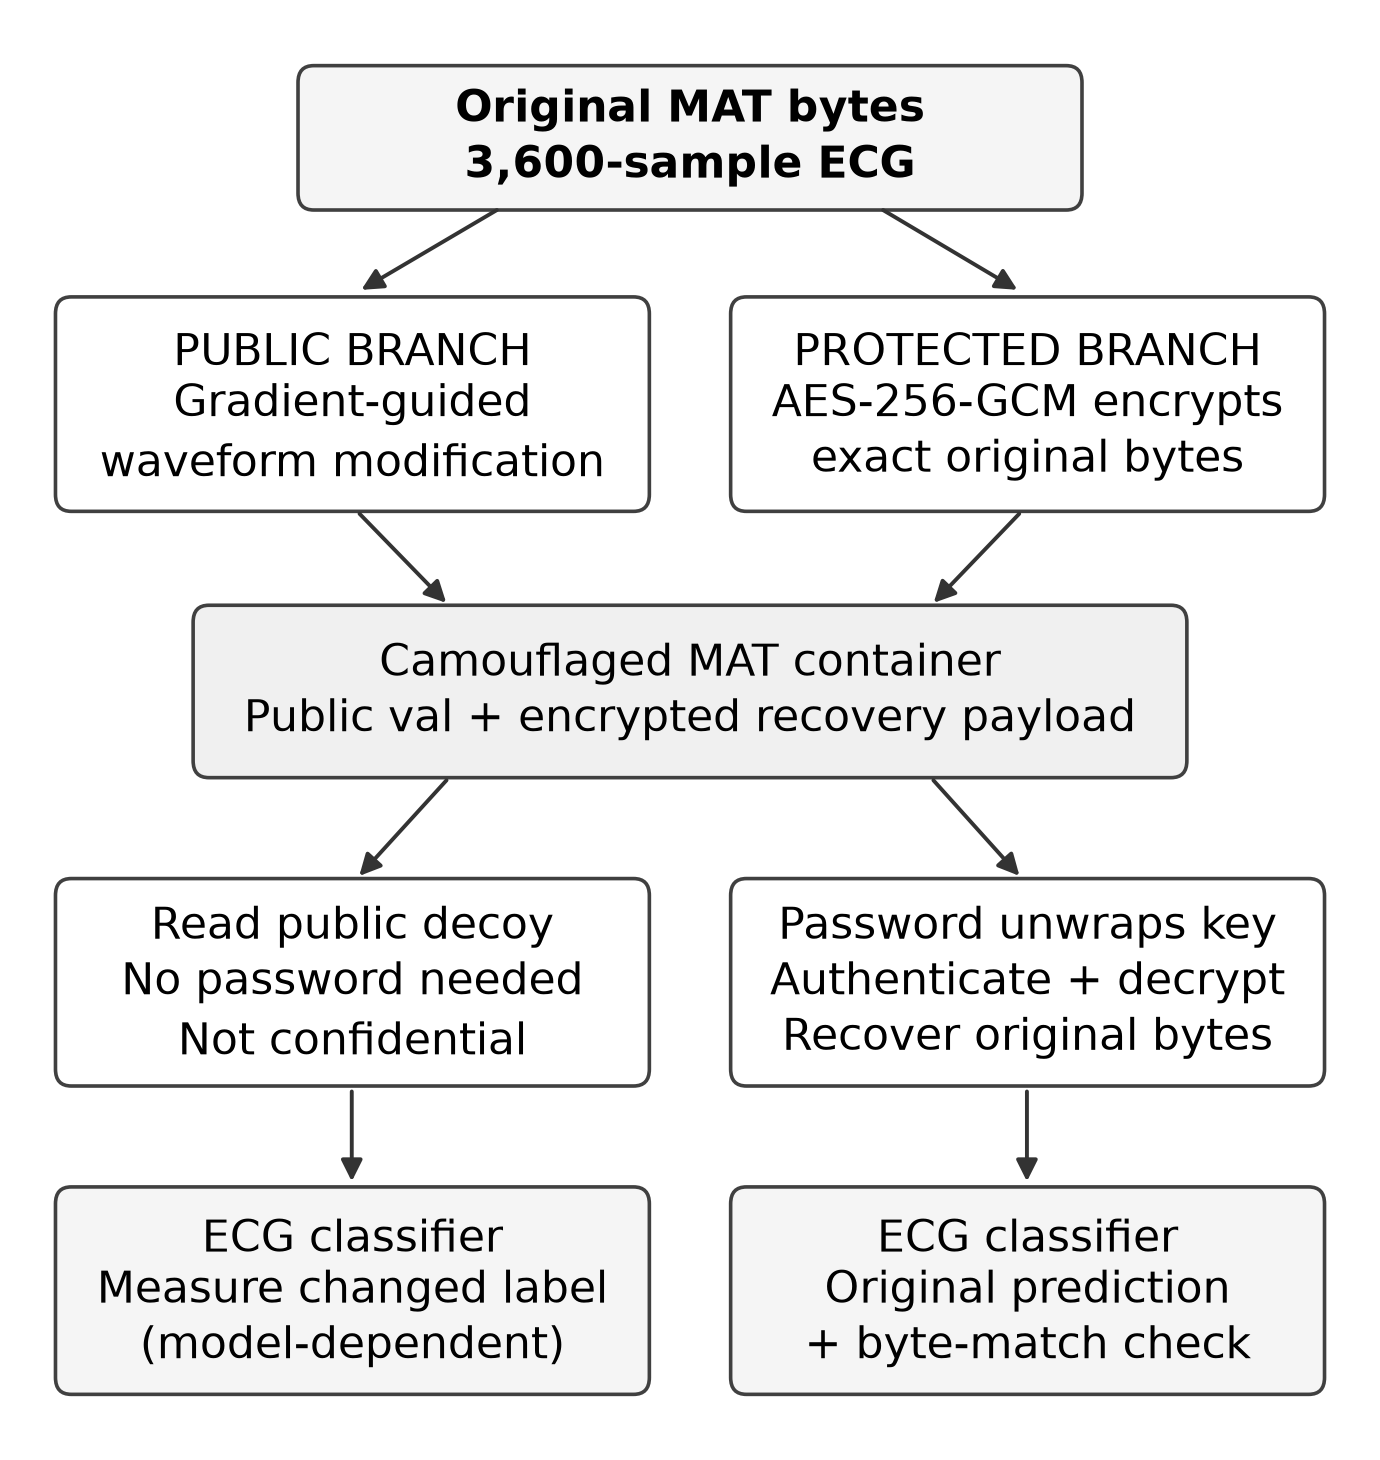
\includegraphics[width=0.88\linewidth]{figures/fig01_workflow.png}
\caption{Public-signal and protected-original paths. Recovery reads the encrypted original payload, not an inverse perturbation. The batch key envelope and authenticated manifest are also required.}\label{fig:workflow}
\end{figure}

The white-box camouflage routine knows the selected classifier and its preprocessing. It tries to change that classifier's original prediction within a raw-amplitude budget. We do not assume that the resulting waveform conceals identity, prevents an attacker from learning clinical information, or transfers to another model. An attacker who can access the plaintext source directory is outside the protection offered by encrypted copies. The prototype runs locally for a trusted user and is not a remotely hardened service.

\subsection{Iterative raw waveform camouflage}

Let $x$ denote the 3,600-sample raw waveform, $P$ the fixed preprocessing operation, and $f$ the classifier. Let $s$ be the scaled median absolute deviation of the band-passed original signal. The raw perturbation budget $b$ and nominal update size $\alpha$ are defined by (\ref{eq:budget}), where $\epsilon_c$ is the camouflage setting and $T$ is the maximum iteration count. Defaults are $\epsilon_c=0.5$ and $T=20$.

\begin{equation} b=\epsilon_c s, \qquad \alpha=2b/T. \label{eq:budget} \end{equation}

At each iteration the routine computes cross-entropy relative to the original predicted class, differentiates in the 900-sample normalized model-input domain, and linearly interpolates that gradient to 3,600 points. Denote the interpolated gradient by $U(g_t)$. The raw candidate update is (\ref{eq:update}), where the projection clips each sample to the interval from $x-b$ to $x+b$.

\begin{equation} x_{t+1}=\Pi_b\!\left(x_t+\alpha\,\operatorname{sign}(U(g_t))\right). \label{eq:update} \end{equation}

Every candidate is run again through the real SciPy preprocessing and classifier. The process stops when the predicted label changes; otherwise the candidate with the lowest original predicted-class softmax score is retained. Bounds are adjusted inward for float32 representation so that rounding does not enlarge the budget. Constant or numerically zero-scale inputs are not modified. Because the method does not differentiate through filtering and median/MAD normalization, it is a gradient-guided heuristic rather than exact raw-space PGD.

Algorithm 1 summarizes the implementation. (1) Read and preserve the original MAT bytes. (2) Measure the original model output and raw budget. (3) Generate projected raw candidates, re-evaluating each candidate through P and f. (4) Record the best actual output and whether its label changed. (5) Encrypt the exact original bytes and bind the public decoy and record context as associated data. (6) Verify exact recovery before publishing the completed batch. A reference label is used for correctness reporting, not to fabricate a changed prediction.

\subsection{File container and key handling}

Each batch receives a random 256-bit AES data key. Original MAT files, rendered waveform PNGs, and the private manifest are encrypted using AES-GCM with fresh 96-bit nonces and 128-bit authentication tags. A password-derived wrapping key protects the batch key. The implementation uses scrypt with N = 131072, r = 8, p = 1, and a random 128-bit salt. The demo intentionally uses the public fixed password 987654321; this configuration is unsuitable for confidential patient data despite the standard encryption primitive.

A camouflaged MAT contains public float32 val samples and an encrypted original-MAT recovery payload, together with a nonce, format version, and batch/record context. Associated data bind the version, context, and canonical little-endian float32 decoy bytes. Altering those bound fields causes authentication failure. Recovery retrieves the original file as bytes, preserving its original MATLAB representation rather than reconstructing it from a rounded waveform array. A complete batch archive is required because an individual container does not include a usable unwrapped key.

The GUI checks MAT and PNG equality and compares source and recovered predictions using the same selected checkpoint. Results and explanation images are encrypted when saved. Before password entry, a grayscale diagnostic can visualize ciphertext byte values; this is not an ECG image input or an authenticity check. Public decoy metadata are similarly unauthenticated until recovery succeeds. Clearing results removes decrypted previews from the interface but does not guarantee secure erasure from browser or operating-system memory.

\subsection{Separate FGSM sensitivity experiment}

The optional FGSM experiment uses a temporary copy of the normalized 900-sample input. It adds $\epsilon_a$ times the sign of the cross-entropy gradient with respect to the reference class \cite{goodfellow2015}. No arbitrary amplitude clipping is applied. $\epsilon_a=0.05$ therefore has different units and a different optimization procedure from $\epsilon_c=0.5$. Neither value is a decryption parameter. Correct restoration depends on the key and authenticated payload, not on matching perturbation settings.

\section{Experimental Results}

\subsection{Internal classification evaluation}

The existing checkpoint correctly classifies 174 of the 200 reconstructed validation fragments. Table~\ref{tab:metrics} provides overall metrics, and Figure~\ref{fig:confusion} shows the confusion matrix. Weighted F1 is 86.22\%, whereas macro F1 is 76.09\%, indicating that the aggregate weighted score masks uneven class behavior. SVTA and Fusion have zero recall. Several other classes have only two to four validation samples, so apparently perfect scores should not be interpreted as reliable estimates for those rhythms.

\begin{table}
\centering
\caption{Leakage-affected internal validation results}\label{tab:metrics}
\small
\begin{tabular}{ll}
\hline
Metric & Value \\
\hline
Correct fragments & 174 / 200 \\
Accuracy & 87.00\% \\
Weighted precision & 86.40\% \\
Weighted recall & 87.00\% \\
Weighted F1 & 86.22\% \\
Macro F1 & 76.09\% \\
Balanced accuracy & 76.79\% \\
Macro OvR ROC AUC & 0.9907 \\
Macro average precision & 0.9151 \\
\hline
\end{tabular}
\end{table}

The macro one-versus-rest ROC AUC of 0.9907 describes ranking of continuous scores, not the accuracy of the maximum-score label. High ranking scores can coexist with low class recall. Model outputs have not been calibrated as clinical probabilities, and no prospective clinical comparison was performed. We do not plot a training/validation learning curve because per-epoch validation history was not saved.

\subsection{FGSM sensitivity of the baseline}

\begin{figure}
\centering
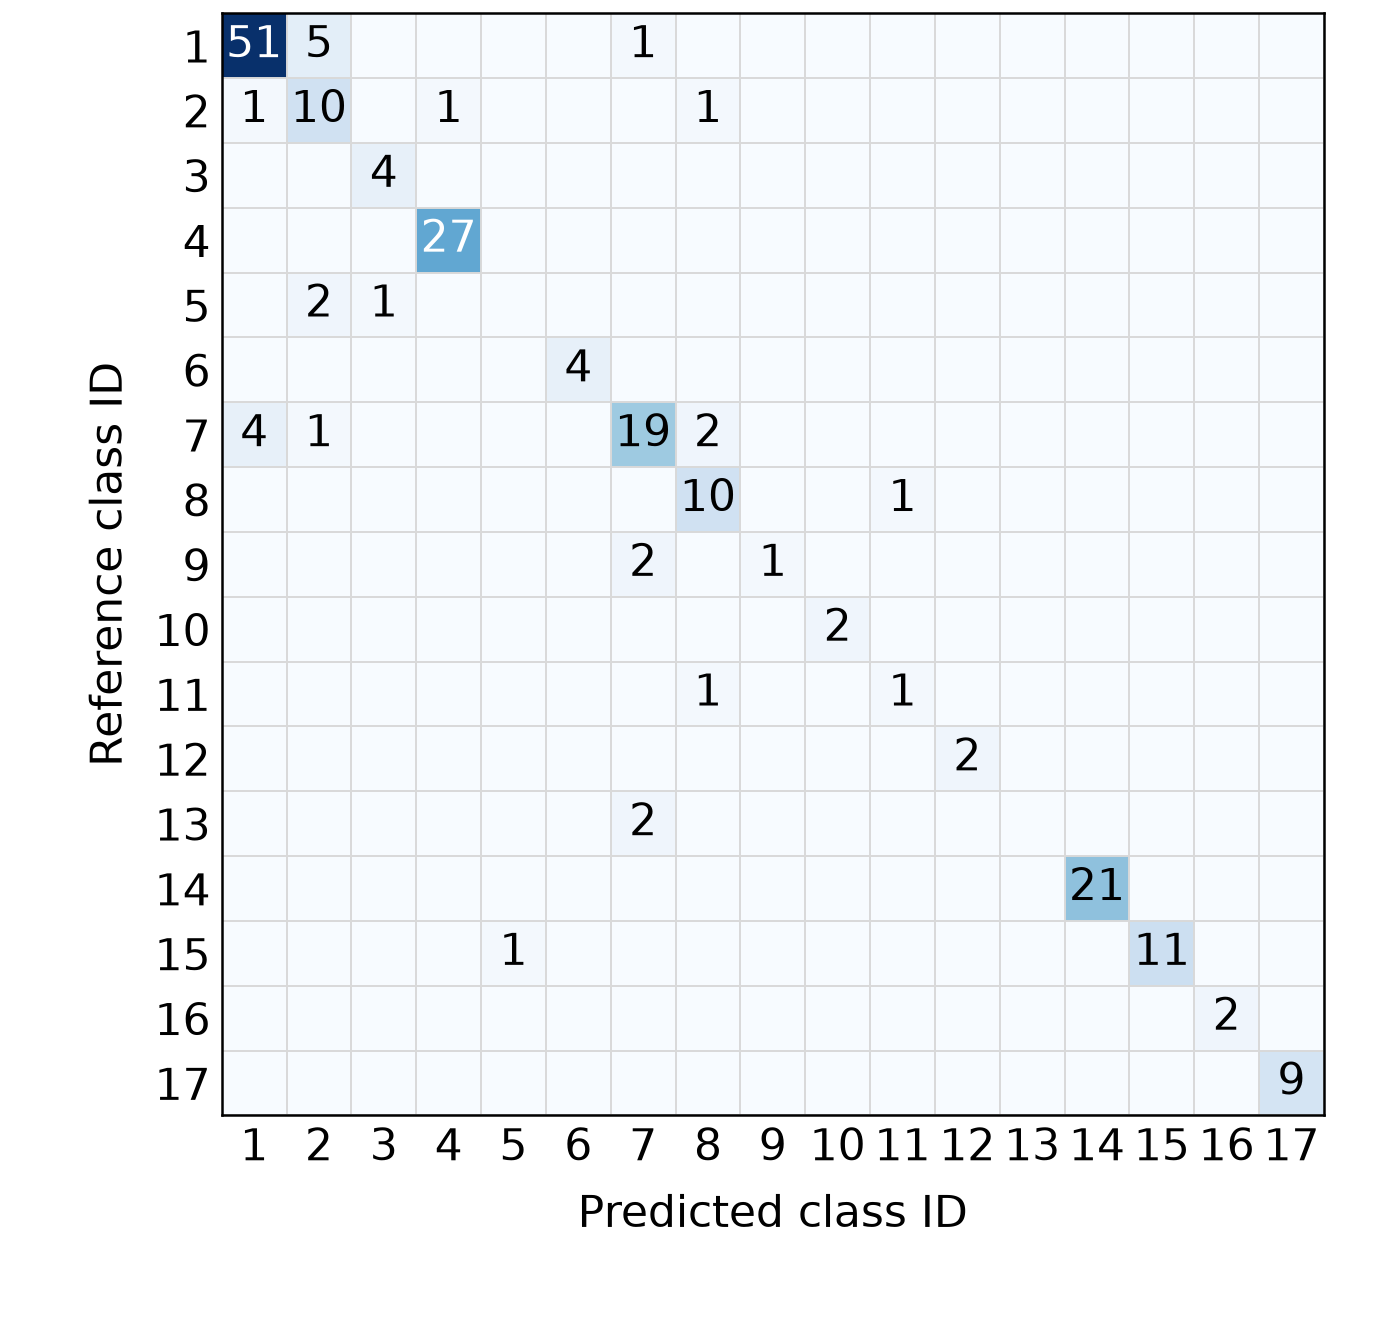
\includegraphics[width=0.88\linewidth]{figures/fig02_confusion_matrix.png}
\caption{Confusion matrix for 200 validation fragments; class IDs follow Table~\ref{tab:support}. Counts sum to 200, with 174 correct. Recording overlap and exact duplicates limit interpretation.}\label{fig:confusion}
\end{figure}

\begin{figure}
\centering
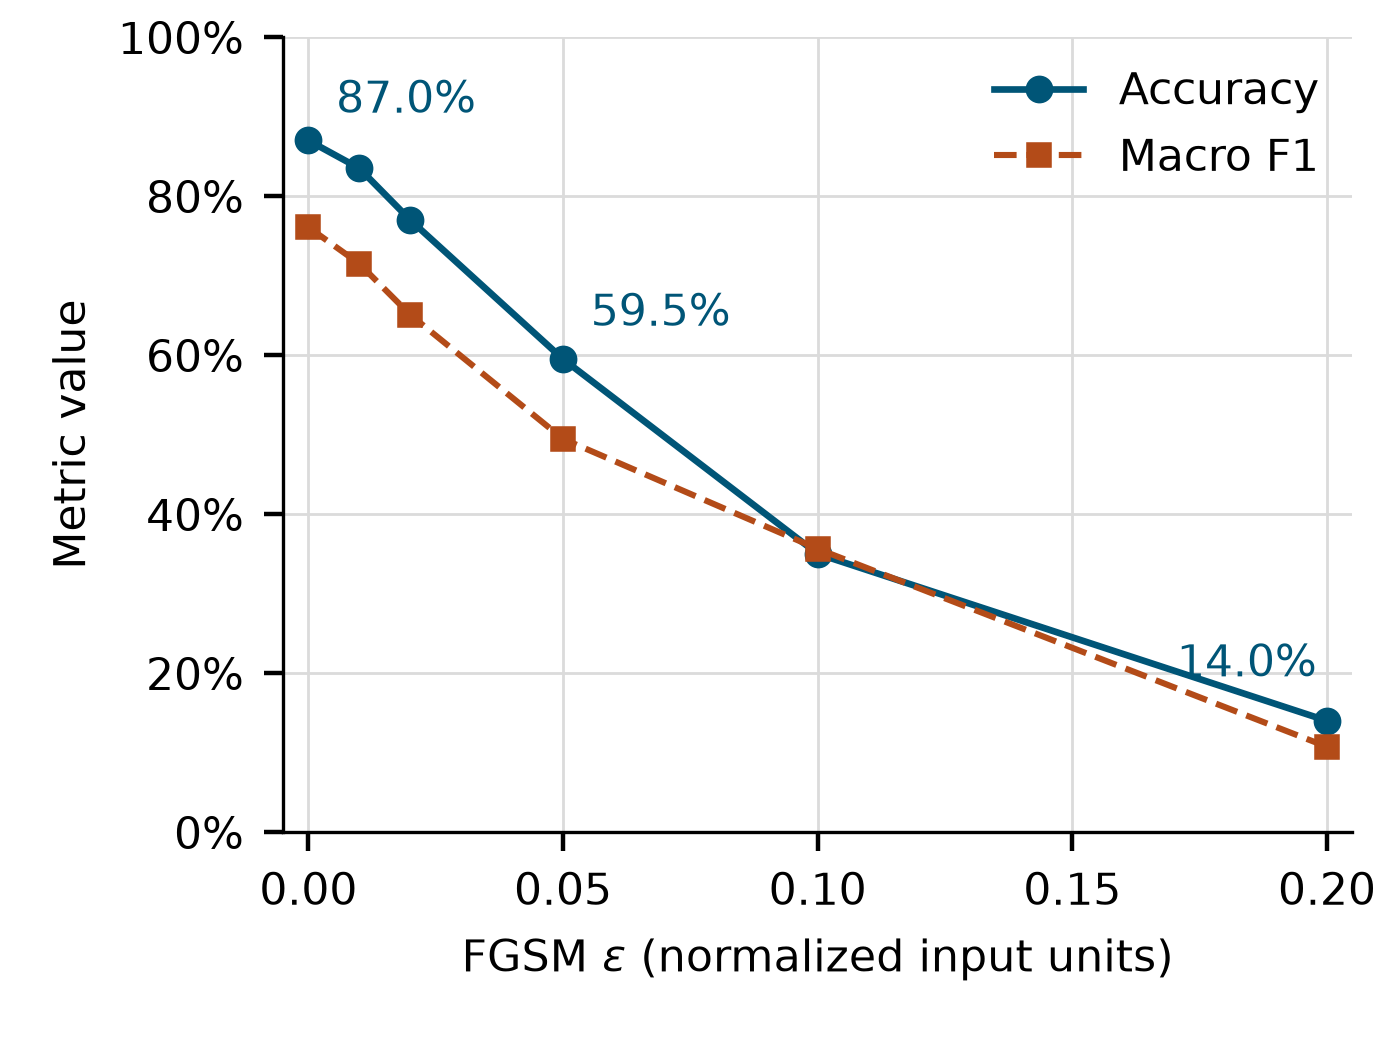
\includegraphics[width=0.88\linewidth]{figures/fig03_fgsm_curve.png}
\caption{Baseline FGSM sensitivity on the reconstructed validation split. Epsilon is measured in normalized input units. This single-attack curve is not a robustness guarantee.}\label{fig:fgsm}
\end{figure}

Figure~\ref{fig:fgsm} and Table~\ref{tab:fgsm} summarize the separate white-box FGSM experiment on the same 200 validation fragments. Accuracy decreases from 87.0\% without perturbation to 59.5\% at $\epsilon_a=0.05$ and 14.0\% at 0.20. The 0.05 setting produces a 27.5-percentage-point absolute decrease. The evaluated model is the original baseline; optional adversarial-training code is available, but those training options are not evidence of an adversarially trained checkpoint in this experiment.

\begin{table}
\centering
\caption{Normalized-input FGSM experiment}\label{tab:fgsm}
\small
\begin{tabular}{lccc}
\hline
Epsilon & Correct / 200 & Accuracy \% & Macro F1 \\
\hline
0.00 & 174 & 87.0 & 0.7609 \\
0.01 & 167 & 83.5 & 0.7150 \\
0.02 & 154 & 77.0 & 0.6507 \\
0.05 & 119 & 59.5 & 0.4946 \\
0.10 & 70 & 35.0 & 0.3563 \\
0.20 & 28 & 14.0 & 0.1074 \\
\hline
\end{tabular}
\end{table}

\subsection{Whole-dataset camouflage and exact recovery}

A completed 1,000-record camouflage batch uses $\epsilon_c=0.5$, at most 20 steps, and the same checkpoint. Its authenticated creation-time reports record label changes for all 1,000 fragments. This is a whole-dataset, model-specific optimization experiment that includes training fragments; it is not an independent attack-prevention rate. Of the original predictions, 969 were correct. All 969 became incorrect after camouflage, while 21 initially incorrect predictions became correct. A label-change count therefore differs from a correctness-based attack-success statistic.

\begin{table}
\centering
\caption{Whole-dataset camouflage and recovery audit}\label{tab:audit}
\small
\begin{tabular}{p{0.61\linewidth}l}
\hline
Quantity & Observed result \\
\hline
Fragments processed & 1,000 \\
Changed predicted labels & 1,000 / 1,000 \\
Original correct $\rightarrow$ incorrect & 969 \\
Original incorrect $\rightarrow$ correct & 21 \\
Iterations used min / median / max & 1 / 2 / 9 \\
Measured raw-budget violations & 0 \\
Exact embedded MAT recovery & 1,000 / 1,000 \\
Recovered MAT matches source & 1,000 / 1,000 \\
\hline
\end{tabular}
\end{table}

Dataset-wide creation-time prediction reports were authenticated without recomputing their predictions; the single Figure~\ref{fig:recovery} example was re-evaluated. Independently, all embedded recovery payloads were decrypted and compared against the separately encrypted original MAT bytes and current source files. All 1,000 comparisons were exact, and every original MAT and PNG plaintext hash matched the authenticated manifest. This establishes byte-preserving recovery for the audited batch; it does not establish that the readable decoys protect privacy.

For Figure~\ref{fig:recovery}, the decoy changes the selected model's prediction from NSR to APB after two iterations. The raw budget is 8.85518 dataset units, the measured maximum change is 1.77100, and decoy-versus-original MSE is 2.37149. Original-versus-restored MSE is zero because recovery is byte exact. This example was selected to illustrate the GUI workflow and belongs to the training split, so it is not presented as held-out evidence.

\subsection{Software verification and reproducibility}

The current regression suite passes 114 tests covering signal loading, prediction, password errors, tamper rejection, path boundaries, public previews, and exact restoration. Tests verify that a locked ciphertext preview needs neither model loading nor decryption and that wrong passwords do not return original data. Automated tests support functional correctness of these cases; they are not a cryptographic security proof, penetration test, or clinical validation.

\begin{figure}
\centering
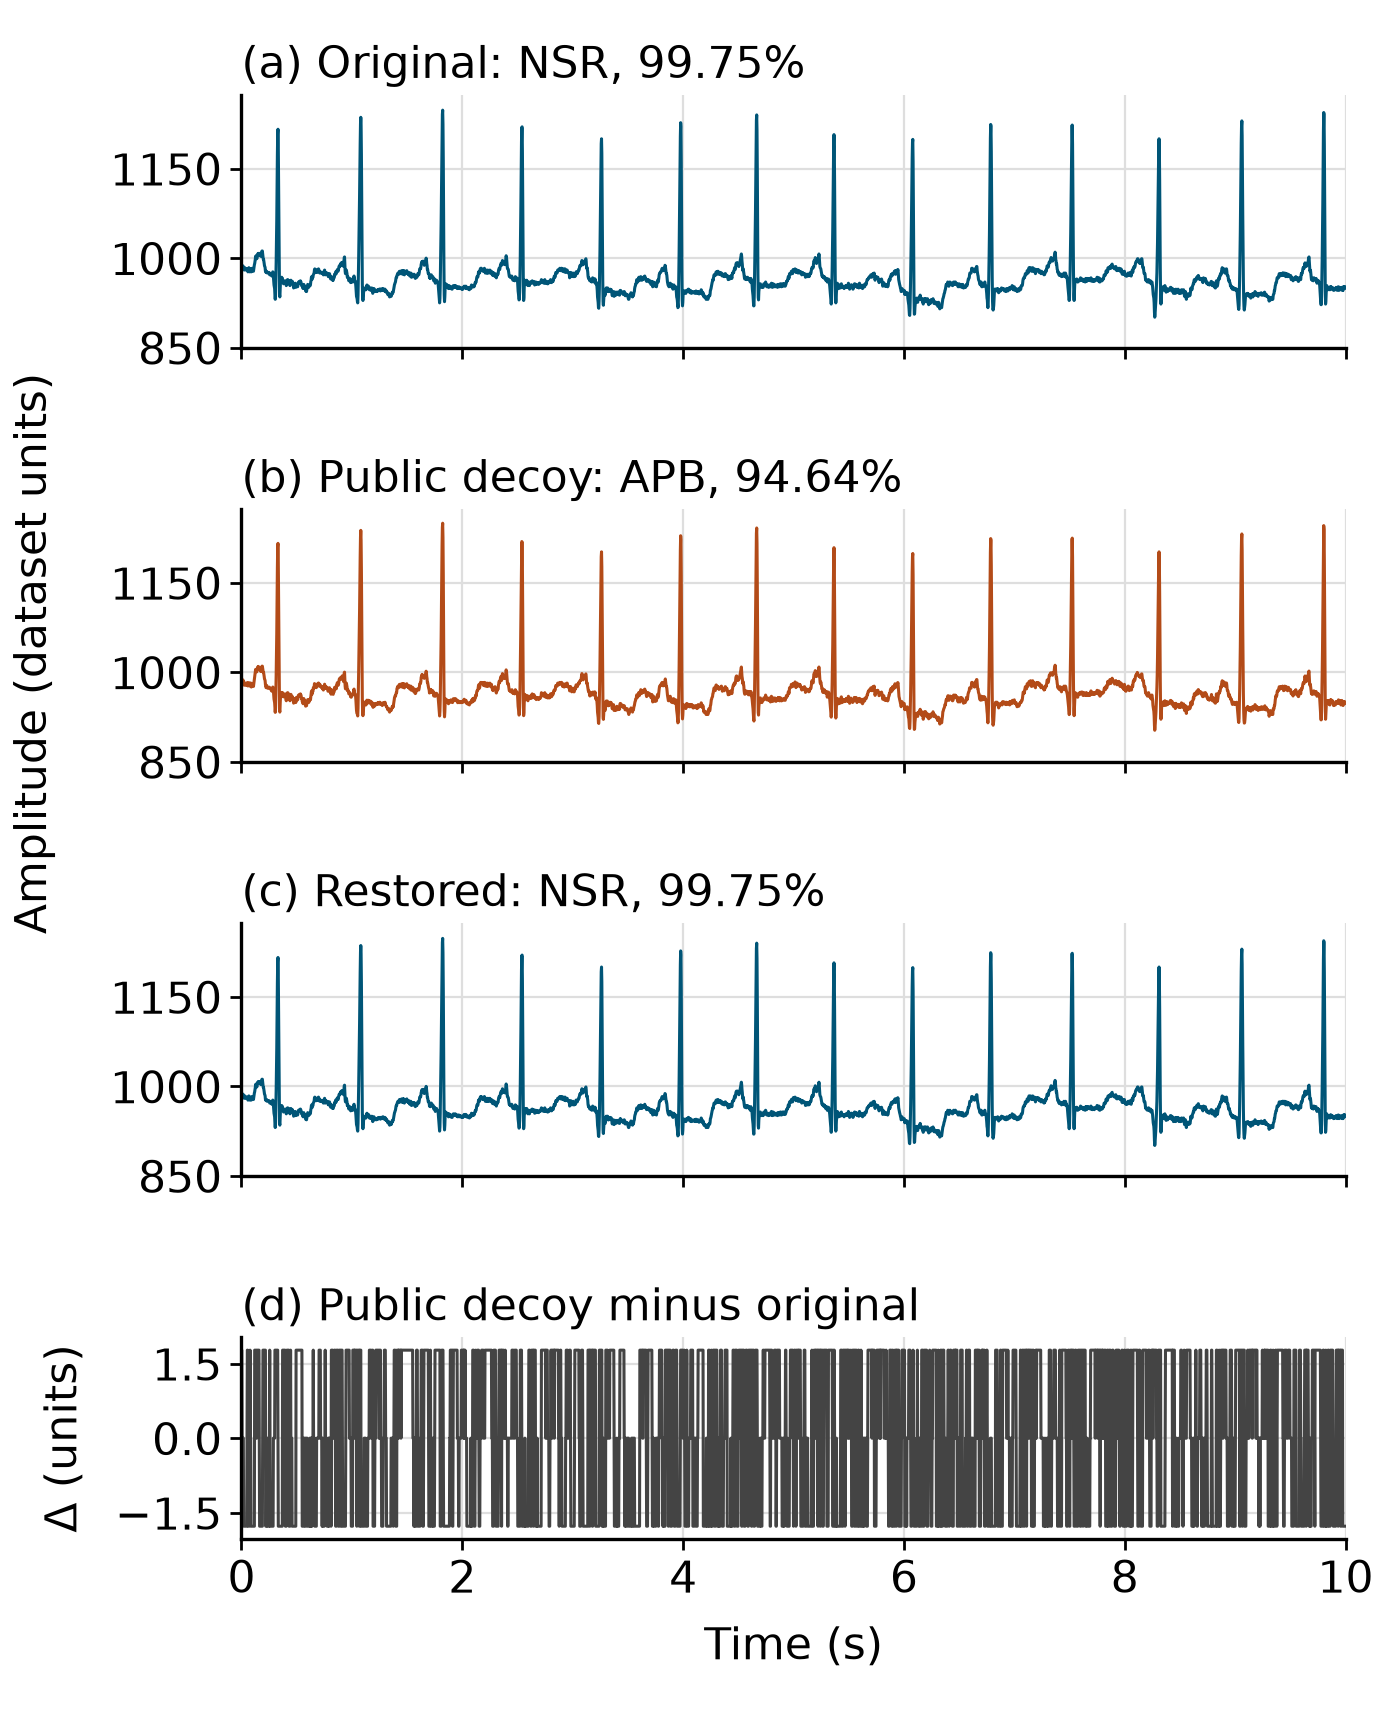
\includegraphics[width=0.88\linewidth]{figures/fig04_camouflage_recovery.png}
\caption{Illustrative training fragment 100m (2).mat: original NSR score 99.75\%, public-decoy APB score 94.64\%, and exact restored original. Waveforms use raw dataset units; the difference panel magnifies the alteration.}\label{fig:recovery}
\end{figure}

Classification figures originate from the saved results.json, split manifest, and validation predictions generated with the existing model. The audited camouflage batch is f5af518e8dc04ebb9bd4504b31c8f052. The checkpoint SHA-256 begins f2ea83714317c0b9; the full digest and batch configuration accompany the manuscript in the reproducibility notes. Reproduction uses the supplied MLII directory, checkpoint, current source code, and scripts. No model was retrained to create this manuscript.

\section{Limitations and Responsible Use}

The strongest limitation is evaluation leakage. A new experiment should group fragments by verified patient or recording identity, remove duplicate waveforms before splitting, and report uncertainty across repeated independent splits. Rare classes require larger support. Current scores are not calibrated, and comparison with established ECG baselines on identical partitions remains outstanding. The results do not support a claim that the prototype diagnoses CVD or estimates individual patient risk.

The threat model is narrow. Camouflage was optimized against one accessible checkpoint, without transfer testing, adaptive reconstruction attacks, membership inference, or clinical-attribute leakage analysis. The public waveform may retain clinically meaningful morphology even if the model changes its label. Fresh nonces and authenticated recovery protect the encrypted payload, but the public fixed password and retained plaintext source directory make the demo inappropriate for private patient records. A deployment would require separate key management, strong user secrets, access controls, and an explicit data-retention policy.

The raw update uses an interpolated model-input gradient rather than an exact derivative through preprocessing. Its budget is relative to a per-record scale and is not a clinical distortion threshold. The FGSM curve samples only one attack family and cannot certify resistance to iterative, black-box, or adaptive attacks. No full RNAF reinforcement-learning policy or defense efficacy is evaluated. These unimplemented components should remain future research, not be described as completed contributions.

The interface includes static, source-linked general care information for the original or restored model label. It never derives care advice from a decoy label, and the dataset contains no treatment or outcome targets. This feature is educational and has not undergone independent clinical validation; treatment selection requires qualified clinical review. Likewise, Grad-CAM and the uncalibrated model scores cannot validate a diagnosis.

\section{Conclusion}

The workbench demonstrates a reproducible separation between adversarial ECG signal manipulation and authenticated exact-original recovery. A compact residual-attention baseline yields 87.00\% accuracy on an internal fragment split, with substantial recording overlap that restricts the claim. The selected camouflage configuration changes all 1,000 recorded predictions, while independent checks recover every original MAT exactly. These findings establish the implemented workflow and its model sensitivity, not attack prevention, anonymization, or clinical readiness. Future evaluation should prioritize leakage-free recording or patient splits, stronger and transferable attacks, calibrated uncertainty, and secure key management before investigating a complete RNAF-inspired adaptive defense.

\begin{thebibliography}{7}
\bibitem{plawiak2017} P. Plawiak, ``ECG signals (1000 fragments),'' Mendeley Data, V3, 2017, doi: 10.17632/7dybx7wyfn.3.
\bibitem{moody2001} G. B. Moody and R. G. Mark, ``The impact of the MIT-BIH Arrhythmia Database,'' \textit{IEEE Eng. Med. Biol. Mag.}, vol. 20, no. 3, pp. 45--50, 2001. Database: PhysioNet, ver. 1.0.0, 2005, doi: 10.13026/C2F305.
\bibitem{rizwan2025} K. Rizwan, M. A. Habib, S. Raza, and M. Ahmad, ``RNAF: ResilienceNet Adversarial Framework Using Deep Reinforcement Learning for Adversarial Attacks on Digital Images,'' \textit{IEEE Access}, vol. 13, pp. 201592--201610, 2025, doi: 10.1109/ACCESS.2025.3636942.
\bibitem{goodfellow2015} I. J. Goodfellow, J. Shlens, and C. Szegedy, ``Explaining and Harnessing Adversarial Examples,'' in \textit{Proc. ICLR}, 2015, arXiv:1412.6572.
\bibitem{madry2018} A. Madry, A. Makelov, L. Schmidt, D. Tsipras, and A. Vladu, ``Towards Deep Learning Models Resistant to Adversarial Attacks,'' in \textit{Proc. ICLR}, 2018, arXiv:1706.06083.
\bibitem{dworkin2007} M. Dworkin, ``Recommendation for Block Cipher Modes of Operation: Galois/Counter Mode (GCM) and GMAC,'' NIST SP 800-38D, Nov. 2007, doi: 10.6028/NIST.SP.800-38D.
\bibitem{selvaraju2019} R. R. Selvaraju, M. Cogswell, A. Das, R. Vedantam, D. Parikh, and D. Batra, ``Grad-CAM: Visual Explanations from Deep Networks via Gradient-Based Localization,'' \textit{Int. J. Comput. Vis.}, 2019, doi: 10.1007/s11263-019-01228-7.
\end{thebibliography}
\end{document}
